\documentclass[12pt]{article}
\usepackage{amsfonts,amssymb,amsmath}
\usepackage{graphicx}
%\documentstyle[12pt,amsfonts]{article}
%\documentstyle{article}

\setlength{\topmargin}{-.5in}
\setlength{\oddsidemargin}{0 in}
\setlength{\evensidemargin}{0 in}
\setlength{\textwidth}{6.5truein}
\setlength{\textheight}{8.5truein}
%\input ../basicmath/basicmathmac.tex
%
%\input ../adgeomcs/lamacb.tex
\input ../Cis515_HW3/mac-new.tex
\input ../Cis515_HW3/mathmac.tex

\def\fseq#1#2{(#1_{#2})_{#2\geq 1}}
\def\fsseq#1#2#3{(#1_{#3(#2)})_{#2\geq 1}}
\def\qleq{\sqsubseteq}

%
\begin{document}
\begin{center}
\fbox{{\Large\bf Fall 2016 \hspace*{0.4cm} CIS 515}}\\
\vspace{1cm}
{\Large\bf Fundamentals of Linear Algebra and Optimization\\
Jean Gallier \\
\vspace{0.5cm}
Homework 3}\\[10pt]
October 25, 2016\\
Francine Leech, Reffat Manzur, Chen Xiang \\
\end{center}


\vspace {0.25cm}\noindent
{\bf Problem B1 (20 pts).} \\
Let us prove this first for two subspaces. $E = U_1 \oplus U_2$ if and only if $$ (1)\ E = U_1  + U_2$$ and $$(2)\ U_1 \cap U_2 = {0}$$. 

For $(1)$, every vector $e \in E$ can be uniquely written as $e = u_{11} + u_{21}$ with $u_{11} \in U_1$ and $u_{21} \in U_2$. \\

For $(2)$, let $e \in U_1 \cap U_2$. Since $e \in U_1$ and $e \in U_2$, then we can write, \\

$(1)\ e = e + 0$ where $e \in U_1$ and $0 \in U_2$ and  \\

$(2)\ e = 0 + 0$ where $0 \in U_1$ and $e \in U_2$.  \\ 

But $e = u_{11} + u_{21}$ is unique, so $e=0$. Since $E = U_1 + U_P$, we will check uniqueness. Suppose $e = u_{11} + u_{21}$ and $e = u_{12} + u_{22}$ where $u_{11} , u_{12}  \in U_1$ and $u_{21} , u_{22}  \in U_2$. Then $u_{11} + u_{21} = u_{12} + u{22}$, so $u_{11} - u_{12} = u_{22} - u_{21}$.  Let $x$ be a vector such that $x = u_{11} - u_{12} = u_{22} - u_{21}$. Then $x \in U_1$ and $x \in U_2$, and $u_{11} = u_{12}$ and $u_{22} = u_{21}$, so $x \in U_1 \cap U_2 = (0)$. \\

Now by induction we can extend our logic for any number of $p\geq 2$  subspaces of some vector space $E$. 



\vspace {0.25cm}\noindent
{\bf Problem B2 (50 pts).}

\medskip
(1)\\

By definition an involution is a function $f$ that is its own inverse. \\

$f: E \rightarrow E$ is in an involution when $\forall x \in E: f(f(x)) = x$. Since $f^{-1} = f$, we just have to check that $f(f(x)) =x$ for all x in the domain of f. \\

Let us find the inverse of $f(x) = b -x$ where b is any real number. Let,  
$$f(x) = a -x$$
$$y=a-x$$
$$f^{-1} = a - y $$
$$ x = a-y$$
$$y= a-x$$
so $f(x) = f^{-1}(x)$. So it's an inverse of itself. \\

\medskip
(2)\\

Let $u_1 = \frac{u + f(u)}{2}$ and $u_{-1} = \frac{u-f(u)}{2}$. \\

Next, we can find that we have something in both the spaces. 
$f(u_1) = f(\frac{u+f(u)}{2}) = \frac{f(u) + f(f(u))}{2} = \frac{f(u) + u}{2} = u_1$ \\
$f(u_{-1}) = f(\frac{u-f(u)}{2}) = \frac{f(u)-f(f(u))}{2} = \frac{f(u) - u}{2} = u_{-1}$. \\

Next we need to look at uniqueness. Let $v_1 \in E_1 and \in E_{-1}$. \\
$f(v_1) = v_1$ \\
$f(v_1) = -v_1$ \\
$v_1 = -v_1$ can only have this if $v_1 = -v_1 = 0$. 



\medskip
(3)
If $E$ is finite-dimensional and $f$ is an involution, prove that
there is some basis of $E$ over which the matrix of $f$ is of the form
\[
I_{k , n - k} =
\begin{pmatrix}
I_k & 0 \\
0 & - I_{n - k}
\end{pmatrix},
\]
where $I_k$ is the $k\times k$ identity matrix 
(similarly for $I_{n -  k}$) and $k = \mathrm{dim}(E_1)$.
Can you give a geometric interpretation of the action of $f$
(especially when   $k = n - 1$)?


\vspace {0.5cm}\noindent
{\bf Problem B3 (50 pts).}
A {\it rotation\/} $R_{\theta}$ in the plane $\reals^2$ is given  by
the matrix
\[
R_{\theta} =
\begin{pmatrix}
\cos\theta & -\sin\theta \\
\sin\theta & \cos\theta
\end{pmatrix}.
\]

\medskip
(1)
Use {\tt Matlab} to show the action of a rotation $R_{\theta}$
on a simple figure such as a triangle or a rectangle,
for various values of $\theta$, including
$\theta = \pi/6, \pi/4, \pi/3, \pi/2$.

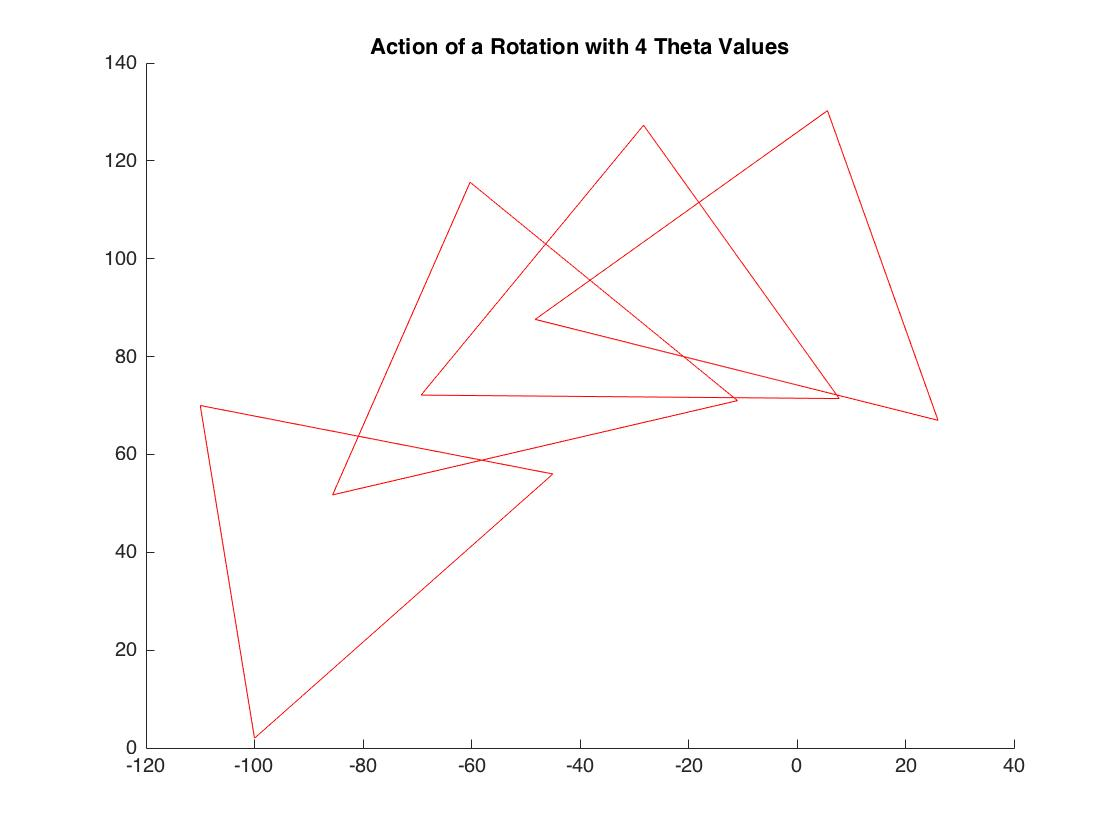
\includegraphics[scale=.25]{RotationPlot}

\medskip
(2)
Prove that $R_{\theta}$ is invertible and that its inverse is
$R_{-\theta}$.

\[
\begin{pmatrix}
\cos\theta & -\sin\theta \\
\sin\theta & \cos\theta
\end{pmatrix}
\cdot
\begin{pmatrix}
\cos(-\theta) & -\sin(-\theta) \\
\sin(-\theta) & \cos(-\theta)
\end{pmatrix}
\]

\[
=
\begin{pmatrix}
\cos(1) & -\sin(1) \\
\sin(1) & \cos(1)
\end{pmatrix}
\cdot
\begin{pmatrix}
\cos(-1) & -\sin(-1) \\
\sin(-1) & \cos(-1)
\end{pmatrix}
\]
\[
=
\begin{pmatrix}
(\cos\theta \cdot \cos(-theta)) \cdot (-\sin\theta \sin(-\theta)) & -\cos(\theta)0 \\
\sin(\theta)cos(-theta)+cos\theta \sin(-\theta) & 1\cos(1)
\end{pmatrix}
=
\begin{pmatrix}
1 & 0 \\
0 & 1
\end{pmatrix}
\]



\medskip
(3) For any two rotations $R_{\alpha}$ and $R_{\beta}$, prove that
\[
R_{\beta}\circ R_{\alpha} = R_{\alpha}\circ R_{\beta} = R_{\alpha + \beta}.
\]

Use (2)-(3) to prove that the rotations in the plane form a commutative
group
denoted $\mathbf{SO}(2)$.

\vspace {0.5cm}\noindent
{\bf Problem B4 (110 pts).}
Consider the affine map $R_{\theta, (a_1,a_2)}$ in $\reals^2$ 
given by
\[
\begin{pmatrix}
y_1 \\
y_2
\end{pmatrix}
=
\begin{pmatrix}
\cos\theta & -\sin\theta \\
\sin\theta & \cos\theta
\end{pmatrix}
\begin{pmatrix}
x_1 \\
x_2
\end{pmatrix}
+ 
\begin{pmatrix}
a_1 \\
a_2
\end{pmatrix}.
\]

\medskip
(1)
Prove that if $\theta\not= k 2\pi$, with $k \in \integs$, then  
$R_{\theta, (a_1,a_2)}$ has
a unique fixed point $(c_1, c_2)$, that is, there is a unique
point  $(c_1, c_2)$ such that
\[
\begin{pmatrix}
c_1 \\
c_2
\end{pmatrix} 
=
R_{\theta, (a_1,a_2)}
\begin{pmatrix}
c_1 \\
c_2
\end{pmatrix}, 
\]
and  this fixed point is given by
\[
\begin{pmatrix}
c_1 \\
c_2
\end{pmatrix} 
=
\frac{1}{2\sin(\theta/2)}
\begin{pmatrix}
\cos(\pi/2 - \theta/2) & -\sin(\pi/2 - \theta/2) \\
\sin(\pi/2 -\theta/2) & \cos(\pi/2 - \theta/2)
\end{pmatrix}
\begin{pmatrix}
a_1 \\
a_2
\end{pmatrix}.
\]

\medskip
(2)
In this question, we still assume that
 $\theta\not= k 2\pi$, with $k \in \integs$.
By translating the coordinate system with origin $(0, 0)$
to the new coordinate system with origin $(c_1, c_2)$, which
means that if $(x_1, x_2)$ are the coordinates with respect to the 
standard origin $(0, 0)$ and if $(x_1', x_2')$ are the coordinates with respect 
to the new origin $(c_1, c_2)$,  we have
\begin{align*}
x_1 & = x_1' + c_1 \\
x_2 & = x_2' + c_2
\end{align*}
and similarly for $(y_1, y_2)$ and $(y_1', y_2')$,
then show that 
\[
\begin{pmatrix}
y_1 \\
y_2
\end{pmatrix} 
=
R_{\theta, (a_1,a_2)}
\begin{pmatrix}
x_1 \\
x_2
\end{pmatrix}
\]
becomes
\[
\begin{pmatrix}
y_1' \\
y_2'
\end{pmatrix} 
=
R_{\theta}
\begin{pmatrix}
x_1' \\
x_2'
\end{pmatrix}.
\]

\medskip
Conclude that with respect to the new origin $(c_1, c_2)$, 
the affine map $R_{\theta, (a_1,a_2)}$ becomes the 
rotation $R_{\theta}$. We say that $R_{\theta, (a_1,a_2)}$ 
is a {\it rotation of center $(c_1, c_2)$\/}.

\medskip
(3)
Use {\tt Matlab} to show the action of  the affine map
$R_{\theta, (a_1,a_2)}$ on a simple figure such as
a triangle or a rectangle,
for $\theta = \pi/3$ and various values of $(a_1, a_2)$.
Display the center $(c_1, c_2)$ of the rotation.

\medskip
What kind of transformations correspond to
$\theta= k 2\pi$, with $k \in \integs$?


\medskip
(4) \\

$R_{\theta, (a_1,a_2)}$ \\
\[
\begin{pmatrix}
y_1 \\
y_2 \\
1
\end{pmatrix}
=
\begin{pmatrix}
\cos\theta & -\sin\theta & a_1 \\
\sin\theta & \cos\theta & a_2 \\
0 & 0 & 1 \\
\end{pmatrix}
\begin{pmatrix}
x_1 \\
x_2 \\
1 \\
\end{pmatrix}
\]

$R_{-\theta, (b_1,b_2)}$ \\
\[
\begin{pmatrix}
y_1 \\
y_2 \\
1
\end{pmatrix}
=
\begin{pmatrix}
\cos(-\theta) & -\sin(-\theta) & b_1 \\
\sin(-\theta) & \cos(-\theta) & b_2 \\
0 & 0 & 1 \\
\end{pmatrix}
\begin{pmatrix}
x_1 \\
x_2 \\
1 \\
\end{pmatrix}
=
\begin{pmatrix}
\cos(\theta) & \sin(\theta) & b_1 \\
-\sin(\theta) & \cos(\theta) & b_2 \\
0 & 0 & 1 \\
\end{pmatrix}
\begin{pmatrix}
x_1 \\
x_2 \\
1 \\
\end{pmatrix}
\] \\

\[
R_{\theta, (a_1,a_2)} \cdot R_{-\theta, (b_1,b_2)} =
\begin{pmatrix}
\cos\theta & -\sin\theta & a_1 \\
\sin\theta & \cos\theta & a_2 \\
0 & 0 & 1 \\
\end{pmatrix}
\begin{pmatrix}
\cos(\theta) & \sin(\theta) & b_1 \\
-\sin(\theta) & \cos(\theta) & b_2 \\
0 & 0 & 1 \\
\end{pmatrix}
\]
\[
=
\begin{pmatrix}
\cos^2\theta + \sin^2\theta & cos\theta \sin\theta - cos\theta \sin\theta & \cos\theta b_1 - \sin \theta b_2 + a_1 \\
cos\theta \sin\theta - cos\theta \sin\theta & \sin^2\theta + \cos^2\theta  & \sin\theta b_1 + \cos\theta b_2 + a_2\\
0 & 0 & 1 \\
\end{pmatrix}
\]
\[
=
\begin{pmatrix}
1 & 0 & 0 \\
0 & 1  & 0 \\
0 & 0 & 1 \\
\end{pmatrix}
\]

So $\cos\theta b_1 - \sin \theta b_2 + a_1 = 0$ and $\sin\theta b_1 + \cos\theta b_2 + a_2 = 0$. \\

Solve for $b_1$, \\
$b_1 = \frac{- a_1 +  \sin \theta b_2}{\cos\theta}$ \\
$b_1 = \frac{- a_1}{\cos\theta} + \frac{\sin \theta b_2}{\cos\theta}$ \\
$b_1 = -\sec\theta a_1 + \tan\theta b_2$ \\

Solve for $b_2$, \\
$b_2 = \frac{- a_2 +  \sin \theta b_1}{\cos\theta}$  \\
$b_2 = \frac{- a_2}{\cos\theta} - \frac{\sin \theta b_1}{\cos\theta}$ \\
$b_2 = \sec\theta a_2 - \tan\theta b_1$ \\

Now plug in $b_2$ into $b_1$.

$b_1 = -\sec\theta a_1 + \tan\theta (\sec\theta a_2 - \tan\theta b_1)$ \\
$b_1 = \sec\theta a_1 - \tan\theta \sec\theta a_2 - \tan^2\theta b_1$ \\
$(1-tan^2\theta)b_1 = \sec\theta a_1 - \tan\theta \sec\theta a_2 $ \\
$b_1 = \frac{-\tan \theta}{\sec \theta}a_2 - \cos \theta a_1$ \\
$b_1 = - \sin \theta a_2 - \cos \theta a_1$ 

Now plug $b_1$ into $b_2$ we get, 
$b_2 = \sin \theta a_1 - \cos \theta a_1$. \\

The final answer for $b_1$ and $b_2$ in terms of $\theta$, $a_1$, and $a_2$ is, 
$$b_1 = -\sin \theta a_2 - \cos \theta a_1$$
$$b_2 = \sin \theta a_1 - \cos \theta a_1$$

\medskip
(5)
Given two affine maps $R_{\alpha, (a_1,a_2)}$ and
$R_{\beta, (b_1,b_2)}$, prove that
\[
R_{\beta, (b_1,b_2)} \circ R_{\alpha, (a_1,a_2)} =
R_{\alpha + \beta, (t_1,t_2)}
\]
for some $(t_1, t_2)$, and find $(t_1, t_2)$ in terms of
$\beta$, $(a_1,a_2)$ and $(b_1,b_2)$.


\medskip
Even in the case where $(a_1,a_2) = (0, 0)$, prove that in general
\[
R_{\beta, (b_1,b_2)} \circ R_{\alpha} \not=
R_{\alpha}  \circ R_{\beta, (b_1,b_2)}. 
\]

Use (4)-(5) to show that the affine maps of the plane defined in this
problem form a nonabelian group denoted $\mathbf{SE}(2)$.

\medskip
Prove that  $R_{\beta, (b_1,b_2)} \circ R_{\alpha, (a_1,a_2)}$ is
not a translation (possibly the identity)  iff
$\alpha + \beta \not= k 2\pi$, for all  $k\in \integs$.
Find its center of rotation when $(a_1, a_2) = (0, 0)$.  

\medskip
If $\alpha + \beta = k 2\pi$, then  $R_{\beta, (b_1,b_2)} \circ
R_{\alpha, (a_1,a_2)}$
is a pure translation. 
Find the translation vector 
of $R_{\beta, (b_1,b_2)} \circ R_{\alpha, (a_1,a_2)}$.


\vspace {0.5cm}\noindent
{\bf Problem B5 (80 pts).}
A subset $\s{A}$ of $\reals^n$ is called an {\it affine subspace\/} if
either $\s{A} = \emptyset$, or there is some vector $a\in \reals^n$
and some subspace $U$ of $\reals^n$ such that
\[
\s{A} = a + U = \{a + u \mid u \in U\}.
\]
We define the dimension $\mathrm{dim}(\s{A})$ of $\s{A}$ as the dimension
$\mathrm{dim}(U)$ of $U$.

\medskip
(1)
If $\s{A} = a + U$, 
why is $a\in \s{A}$?

\medskip
What are affine subspaces of dimension $0$?
What are affine subspaces of dimension $1$ (begin with $\reals^2$)?
What are affine subspaces of dimension $2$ (begin with $\reals^3$)?

\medskip
Prove that any nonempty affine subspace is closed under affine
combinations.

\medskip
(2) Prove that if $\s{A} = a + U$ is any nonempty affine subspace, then
$\s{A} = b + U$ for any $b\in \s{A}$.

\medskip
(3)
Let $\s{A}$ be any nonempty subset of $\reals^n$ closed under affine
combinations.
For any $a\in \s{A}$, prove that 
\[
U_a = \{x - a \in \reals^n \mid x\in \s{A}\} 
\]
is a (linear) subspace of $\reals^n$ such that
\[
\s{A} = a + U_a.
\]
Prove that $U_a$ does not depend on the choice of $a \in \s{A}$; that
is, $U_a = U_b$ for all $a, b\in \s{A}$. In fact, prove that
\[
U_a = U = \{y - x \in \reals^n \mid x, y\in \s{A}\},\quad
\hbox{for all $a\in \s{A}$},
\]
and so
\[
\s{A} = a + U, \quad\hbox{for any $a\in \s{A}$}.
\]

\medskip

\remark
The subspace $U$ is called the {\it direction\/} of $\s{A}$.

\medskip
(4)
Two nonempty affine subspaces $\s{A}$ and $\s{B}$ are said to be {\it
  parallel\/} iff they have the same direction. Prove that that if
$\s{A} \not= \s{B}$ and $\s{A}$ and $\s{B}$ are parallel, then
$\s{A}\cap \s{B} = \emptyset$.

\medskip

\remark
The above shows that
affine subspaces behave quite differently from linear subspaces.



\vspace {0.25cm}\noindent
{\bf Problem B6 (120 pts).} (Affine frames and affine maps)
For any vector $v = (v_1, \ldots, v_n) \in \reals^n$, let 
$\widehat{v}\in \reals^{n+1}$ be the vector 
$\widehat{v} = (v_1, \ldots, v_n,1)$. 
Equivalently, 
$\widehat{v} = (\widehat{v}_1, \ldots, \widehat{v}_{n+1})\in \reals^{n+1}$
is the vector defined by
\[
\widehat{v}_i=
\begin{cases}
v_i & \text{if $1\leq i \leq n$}, \\
1 & \text{if $i = n + 1$}.
\end{cases}
\]

(1)
For any $m + 1$ vectors $(u_0, u_1, \ldots, u_{m })$ 
with $u_i \in \reals^n$  and  $m \leq n$, prove that
if the $m$ vectors $(u_1 - u_0, \ldots, u_m - u_0)$ are linearly
independent, then the $m + 1$ vectors
$(\widehat{u}_0, \ldots,  \widehat{u}_m)$ are linearly independent.

\medskip
(2) Prove that if  the $m + 1$ vectors
$(\widehat{u}_0,  \ldots,  \widehat{u}_m)$ are linearly independent,
then
for any choice of $i$, with $0 \leq i \leq m$, the
$m$ vectors $u_j - u_i$  for $j \in \{0, \ldots, m\}$ with $j - i \not = 0$
are linearly independent.

\medskip
Any $m + 1$ vectors  $(u_0, u_1, \ldots, u_{m })$ such that
the  $m + 1$ vectors
$(\widehat{u}_0, \ldots,  \widehat{u}_m)$ are linearly independent
are said to be {\it affinely independent\/}.

\medskip
From (1) and (2), the vector $(u_0, u_1, \ldots, u_{m })$ 
are affinely independent iff
for any  any choice of $i$, with $0 \leq i \leq m$, the
$m$ vectors $u_j - u_i$  for $j \in \{0, \ldots, m\}$ with $j - i \not = 0$
are linearly independent.
If $m = n$,  we say that $n + 1$ affinely independent 
vectors  $(u_0, u_1, \ldots, u_{n })$ form an {\it affine frame\/} of $\reals^n$. 

\medskip
(3) if $(u_0, u_1, \ldots, u_{n })$ is an affine frame of $\reals^n$,
then prove that for every vector $v\in \reals^n$,  
there is a unique $(n + 1)$-tuple
$(\lambda_0, \lambda_1, \ldots, \lambda_n)\in \reals^{n + 1}$, with
$\lambda_0 + \lambda_1 + \cdots + \lambda_n = 1$, such that
\[
v = \lambda_0 u_0 + \lambda_1 u_1 + \cdots + \lambda_n u_n.
\]
The scalars $(\lambda_0, \lambda_1, \ldots, \lambda_n)$ are called the
{\it barycentric\/} (or {\it affine\/}) {\it coordinates\/} of $v$
w.r.t. the affine frame   $(u_0, u_1, \ldots, u_{n })$.

\medskip
If we write $e_i = u_i -  u_0$, for $i = 1, \ldots, n$, then prove that
we have
\[
v = u_0 + \lambda_1 e_1 + \cdots + \lambda_n e_n,
\]
and since $(e_1, \ldots, e_n)$ is a basis of $\reals^n$ (by (1) \&
(2)), the $n$-tuple $(\lambda_1, \ldots, \lambda_n)$ consists of the 
standard coordinates of $v - u_0$ over the basis $(e_1, \ldots, e_n)$.

\medskip
Conversely, for any vector $u_0\in \reals^n$ and for any basis
$(e_1, \ldots, e_n)$ of $\reals^n$, let
$u_i = u_0 + e_i$ for $i = 1, \ldots, n$. Prove
that $(u_0, u_1, \ldots, u_n)$ is an affine frame of $\reals^n$, 
and for any $v\in \reals^n$, if  
\[
v = u_0 + x_1 e_1 + \dots + x_n e_n,
\]
with $(x_1, \ldots, x_n) \in \reals^n$ (unique), then
\[
v = (1 - (x_1 + \cdots + x_x)) u_0 + x_1 u_1 + \cdots + x_n u_n,
\]
so that $(1 - (x_1 + \cdots + x_x)), x_1, \cdots,  x_n)$,
are the barycentric coordinates of $v$ w.r.t. the affine frame
$(u_0, u_1, \ldots, u_n)$.

\medskip
The above shows that there is a one-to-one correspondence between
affine frames $(u_0, \ldots$, $u_n)$ and pairs
$(u_0, (e_1, \ldots, e_n))$, with  $(e_1, \ldots, e_n)$  a basis.
Given  an affine frame  $(u_0, \ldots, u_n)$, we obtain the basis
$(e_1, \ldots, e_n)$ with $e_i = u_i - u_0$, for $i = 1, \ldots, n$;
given the pair $(u_0, (e_1, \ldots$, $e_n))$ where  $(e_1, \ldots, e_n)$
is a basis,  we obtain the affine frame   $(u_0, \ldots, u_n)$, with
$u_i = u_0 + e_i$, for $i = 1, \ldots, n$.
There is also a  one-to-one correspondence between
barycentric coordinates w.r.t. the affine frame
$(u_0, \ldots, u_n)$ and standard coordinates w.r.t.
the basis   $(e_1, \ldots, e_n)$.
The barycentric cordinates $(\lambda_0, \lambda_1, \ldots, \lambda_n)$
of $v$
(with $\lambda_0 + \lambda_1 + \cdots + \lambda_n = 1$) 
yield the standard coordinates $(\lambda_1, \ldots, \lambda_n)$ of $v - u_0$;
the standard coordinates $(x_1, \ldots, x_n)$ of $v - u_0$ yield the 
barycentric coordinates $(1 - (x_1 + \cdots + x_n ), x_1, \ldots,
x_n)$ of $v$.

\medskip
(4) 
Let $(u_0, \ldots, u_n)$ be any affine frame in $\reals^n$
and let $(v_0, \ldots, v_n)$ be any vectors in $\reals^m$. Prove that there is a {\it
  unique\/} affine map $\mapdef{f}{\reals^n}{\reals^m}$ such that
\[
f(u_i) = v_i, \quad i = 0 , \ldots, n.
\]

\medskip
(5)
Let $(a_0, \ldots, a_n)$ be any affine frame in $\reals^n$ and
let $(b_0, \ldots, b_n)$ be any $n + 1$ points in $\reals^n$. Prove that
the $(n + 1)\times (n + 1)$ matrix $A$ corresponding to
the unique affine map $f$
such that 
\[
f(a_i) = b_i, \quad i = 0, \ldots, n, 
\]
is given by
\[
A = 
\begin{pmatrix}
\widehat{b}_0 & \widehat{b}_1 & \cdots & \widehat{b}_n   
\end{pmatrix}
\begin{pmatrix}
\widehat{a}_0 & \widehat{a}_1 & \cdots & \widehat{a}_n   
\end{pmatrix}^{-1}.
\]

In the special case where  
$(a_0, \ldots, a_n)$ is the canonical  affine frame with 
$a_i = e_{i+1}$ for $i = 0, \ldots, n - 1$ and
$a_n = (0, \ldots, 0)$ 
(where $e_i$ is the $i$th canonical  basis vector), show that
\[
\begin{pmatrix}
\widehat{a}_0 & \widehat{a}_1 & \cdots & \widehat{a}_n   
\end{pmatrix}
= 
\begin{pmatrix}
1  & 0 & \cdots & 0 & 0 \\
0  & 1 & \cdots & 0 & 0\\
\vdots & \vdots & \ddots & 0 & 0 \\
0  &  0  & \cdots & 1 & 0 \\
1  &  1  & \cdots & 1 & 1
\end{pmatrix}
\] 
and
\[
\begin{pmatrix}
\widehat{a}_0 & \widehat{a}_1 & \cdots & \widehat{a}_n   
\end{pmatrix}^{-1}
= 
\begin{pmatrix}
1  & 0 & \cdots & 0 & 0\\
0  & 1 & \cdots & 0 & 0\\
\vdots & \vdots & \ddots & 0 & 0 \\
0  &  0  & \cdots & 1 & 0 \\
-1  &  -1  & \cdots & -1 & 1
\end{pmatrix} .
\]

For example, when $n = 2$, if we write $b_i = (x_i, y_i)$, then
we have
\[
A = 
\begin{pmatrix}
x_1 & x_2 & x_3 \\
y_1 & y_2&  y_3 \\
1  &   1 & 1
\end{pmatrix} 
\begin{pmatrix}
1 & 0 & 0 \\
0 & 1 & 0\\
-1 & -1 & 1
\end{pmatrix} 
= 
\begin{pmatrix}
x_1 - x_3 & x_2 -x_3 & x_3 \\
y_1 - y_3 & y_2 - y_3 &  y_3 \\
0  &   0 & 1
\end{pmatrix} .
\]

\medskip
(6)
Recall that a nonempty affine subspace $\s{A}$ of $\reals^n$ is 
any nonempty subset of  $\reals^n$ closed under affine combinations.
For any affine map $\mapdef{f}{\reals^n}{\reals^m}$, for any
affine subspace $\s{A}$ of $\reals^n$, and any affine subspace $\s{B}$ of
$\reals^m$, prove that $f(\s{A})$ is an affine subspace of $\reals^m$, and that
$f^{-1}(\s{B})$ is an affine subspace of $\reals^n$.



\vspace {0.25cm}\noindent
{\bf Problem B7 (30 pts).} 
Let $A$ be any $n\times k$ matrix

\medskip
(1)
Prove that the $k\times k$ matrix  $\transpos{A} A$ and the matrix $A$
have the same nullspace. Use this  to  prove that 
$\mathrm{rank}(\transpos{A} A) = \mathrm{rank}(A)$.
Similarly, prove that the $n\times n$ matrix  $A\transpos{A}$ and the
matrix $\transpos{A}$
have the same nullspace, and conclude that
$\mathrm{rank}(A\transpos{A}) = \mathrm{rank}(\transpos{A})$.

\medskip
We will prove later that
$\mathrm{rank}(\transpos{A}) =  \mathrm{rank}(A)$.

\medskip
(2)
Let $a_1, \ldots, a_k$ be $k$ linearly independent vectors in $\reals^n$
($1 \leq k \leq n$), and let $A$ be the $n\times k$ matrix whose $i$th
column is $a_i$.
Prove that $\transpos{A}A$ has rank $k$, and that it is
invertible. Let $P = A(\transpos{A}A)^{-1} \transpos{A}$ (an $n\times n$ matrix).
Prove that
\begin{align*}
P^2 & = P \\
\transpos{P} & = P.
\end{align*} 

What is the matrix $P$ when $k = 1$?

\medskip
(3)
Prove that the image of $P$ is the subspace $V$ spanned by
$a_1, \ldots, a_k$, or equivalently the set of all vectors in $\reals^n$
of the form $A x$, with $x\in \reals^k$.
Prove that the nullspace $U$ of $P$ is the set  of vectors $u\in
\reals^n$  such that
$\transpos{A} u = 0$.
Can you give a geometric interpretation of $U$?

\medskip
Conclude that $P$ is a projection of $\reals^n$ onto the
subspace $V$ spanned by $a_1, \ldots, a_k$, and that
\[
\reals^n = U \oplus V.
\]

\hint 
You may use results  from HW2.

\vspace{0.5cm}\noindent
{\bf TOTAL:  460 points.}

\end{document}
